% Options for packages loaded elsewhere
\PassOptionsToPackage{unicode}{hyperref}
\PassOptionsToPackage{hyphens}{url}
\PassOptionsToPackage{dvipsnames,svgnames,x11names}{xcolor}
%
\documentclass[
]{article}
\usepackage{amsmath,amssymb}
\usepackage{iftex}
\ifPDFTeX
  \usepackage[T1]{fontenc}
  \usepackage[utf8]{inputenc}
  \usepackage{textcomp} % provide euro and other symbols
\else % if luatex or xetex
  \usepackage{unicode-math} % this also loads fontspec
  \defaultfontfeatures{Scale=MatchLowercase}
  \defaultfontfeatures[\rmfamily]{Ligatures=TeX,Scale=1}
\fi
\usepackage{lmodern}
\ifPDFTeX\else
  % xetex/luatex font selection
\fi
% Use upquote if available, for straight quotes in verbatim environments
\IfFileExists{upquote.sty}{\usepackage{upquote}}{}
\IfFileExists{microtype.sty}{% use microtype if available
  \usepackage[]{microtype}
  \UseMicrotypeSet[protrusion]{basicmath} % disable protrusion for tt fonts
}{}
\makeatletter
\@ifundefined{KOMAClassName}{% if non-KOMA class
  \IfFileExists{parskip.sty}{%
    \usepackage{parskip}
  }{% else
    \setlength{\parindent}{0pt}
    \setlength{\parskip}{6pt plus 2pt minus 1pt}}
}{% if KOMA class
  \KOMAoptions{parskip=half}}
\makeatother
\usepackage{xcolor}
\usepackage[margin=1in]{geometry}
\usepackage{color}
\usepackage{fancyvrb}
\newcommand{\VerbBar}{|}
\newcommand{\VERB}{\Verb[commandchars=\\\{\}]}
\DefineVerbatimEnvironment{Highlighting}{Verbatim}{commandchars=\\\{\}}
% Add ',fontsize=\small' for more characters per line
\usepackage{framed}
\definecolor{shadecolor}{RGB}{248,248,248}
\newenvironment{Shaded}{\begin{snugshade}}{\end{snugshade}}
\newcommand{\AlertTok}[1]{\textcolor[rgb]{0.94,0.16,0.16}{#1}}
\newcommand{\AnnotationTok}[1]{\textcolor[rgb]{0.56,0.35,0.01}{\textbf{\textit{#1}}}}
\newcommand{\AttributeTok}[1]{\textcolor[rgb]{0.13,0.29,0.53}{#1}}
\newcommand{\BaseNTok}[1]{\textcolor[rgb]{0.00,0.00,0.81}{#1}}
\newcommand{\BuiltInTok}[1]{#1}
\newcommand{\CharTok}[1]{\textcolor[rgb]{0.31,0.60,0.02}{#1}}
\newcommand{\CommentTok}[1]{\textcolor[rgb]{0.56,0.35,0.01}{\textit{#1}}}
\newcommand{\CommentVarTok}[1]{\textcolor[rgb]{0.56,0.35,0.01}{\textbf{\textit{#1}}}}
\newcommand{\ConstantTok}[1]{\textcolor[rgb]{0.56,0.35,0.01}{#1}}
\newcommand{\ControlFlowTok}[1]{\textcolor[rgb]{0.13,0.29,0.53}{\textbf{#1}}}
\newcommand{\DataTypeTok}[1]{\textcolor[rgb]{0.13,0.29,0.53}{#1}}
\newcommand{\DecValTok}[1]{\textcolor[rgb]{0.00,0.00,0.81}{#1}}
\newcommand{\DocumentationTok}[1]{\textcolor[rgb]{0.56,0.35,0.01}{\textbf{\textit{#1}}}}
\newcommand{\ErrorTok}[1]{\textcolor[rgb]{0.64,0.00,0.00}{\textbf{#1}}}
\newcommand{\ExtensionTok}[1]{#1}
\newcommand{\FloatTok}[1]{\textcolor[rgb]{0.00,0.00,0.81}{#1}}
\newcommand{\FunctionTok}[1]{\textcolor[rgb]{0.13,0.29,0.53}{\textbf{#1}}}
\newcommand{\ImportTok}[1]{#1}
\newcommand{\InformationTok}[1]{\textcolor[rgb]{0.56,0.35,0.01}{\textbf{\textit{#1}}}}
\newcommand{\KeywordTok}[1]{\textcolor[rgb]{0.13,0.29,0.53}{\textbf{#1}}}
\newcommand{\NormalTok}[1]{#1}
\newcommand{\OperatorTok}[1]{\textcolor[rgb]{0.81,0.36,0.00}{\textbf{#1}}}
\newcommand{\OtherTok}[1]{\textcolor[rgb]{0.56,0.35,0.01}{#1}}
\newcommand{\PreprocessorTok}[1]{\textcolor[rgb]{0.56,0.35,0.01}{\textit{#1}}}
\newcommand{\RegionMarkerTok}[1]{#1}
\newcommand{\SpecialCharTok}[1]{\textcolor[rgb]{0.81,0.36,0.00}{\textbf{#1}}}
\newcommand{\SpecialStringTok}[1]{\textcolor[rgb]{0.31,0.60,0.02}{#1}}
\newcommand{\StringTok}[1]{\textcolor[rgb]{0.31,0.60,0.02}{#1}}
\newcommand{\VariableTok}[1]{\textcolor[rgb]{0.00,0.00,0.00}{#1}}
\newcommand{\VerbatimStringTok}[1]{\textcolor[rgb]{0.31,0.60,0.02}{#1}}
\newcommand{\WarningTok}[1]{\textcolor[rgb]{0.56,0.35,0.01}{\textbf{\textit{#1}}}}
\usepackage{longtable,booktabs,array}
\usepackage{calc} % for calculating minipage widths
% Correct order of tables after \paragraph or \subparagraph
\usepackage{etoolbox}
\makeatletter
\patchcmd\longtable{\par}{\if@noskipsec\mbox{}\fi\par}{}{}
\makeatother
% Allow footnotes in longtable head/foot
\IfFileExists{footnotehyper.sty}{\usepackage{footnotehyper}}{\usepackage{footnote}}
\makesavenoteenv{longtable}
\usepackage{graphicx}
\makeatletter
\def\maxwidth{\ifdim\Gin@nat@width>\linewidth\linewidth\else\Gin@nat@width\fi}
\def\maxheight{\ifdim\Gin@nat@height>\textheight\textheight\else\Gin@nat@height\fi}
\makeatother
% Scale images if necessary, so that they will not overflow the page
% margins by default, and it is still possible to overwrite the defaults
% using explicit options in \includegraphics[width, height, ...]{}
\setkeys{Gin}{width=\maxwidth,height=\maxheight,keepaspectratio}
% Set default figure placement to htbp
\makeatletter
\def\fps@figure{htbp}
\makeatother
\setlength{\emergencystretch}{3em} % prevent overfull lines
\providecommand{\tightlist}{%
  \setlength{\itemsep}{0pt}\setlength{\parskip}{0pt}}
\setcounter{secnumdepth}{5}
\ifLuaTeX
  \usepackage{selnolig}  % disable illegal ligatures
\fi
\IfFileExists{bookmark.sty}{\usepackage{bookmark}}{\usepackage{hyperref}}
\IfFileExists{xurl.sty}{\usepackage{xurl}}{} % add URL line breaks if available
\urlstyle{same}
\hypersetup{
  pdftitle={Ejercicios Tema 2 - Variables aleatorias. Parte 1 discretas},
  pdfauthor={Ricardo Alberich, Juan Gabriel Gomila y Arnau Mir},
  colorlinks=true,
  linkcolor={Maroon},
  filecolor={Maroon},
  citecolor={Blue},
  urlcolor={Blue},
  pdfcreator={LaTeX via pandoc}}

\title{Ejercicios Tema 2 - Variables aleatorias. Parte 1 discretas}
\author{Ricardo Alberich, Juan Gabriel Gomila y Arnau Mir}
\date{Curso de Probabilidad y Variables Aleatorias con R y Python}

\begin{document}
\maketitle

{
\hypersetup{linkcolor=blue}
\setcounter{tocdepth}{4}
\tableofcontents
}
\hypertarget{variables-aleatorias-discretas}{%
\section{Variables aleatorias
discretas}\label{variables-aleatorias-discretas}}

\hypertarget{problema-1.}{%
\subsection{Problema 1.}\label{problema-1.}}

Hay 10 estudiantes inscritos en una clase de Estadística, de entre los
cuales 3 tienen 19 años, 4 tienen 20 años, 1 tiene 21 años, 1 tiene 24
años y 1 tiene 26 años. De esta clase se seleccionan dos estudiantes sin
reposición. Sea \(X\) la edad media de los dos estudiantes
seleccionados. Hallar la función de probabilidad para \(X\).

\hypertarget{soluciuxf3n}{%
\subsubsection{Solución}\label{soluciuxf3n}}

Los valores que puede alcanzar \(X\) son los siguientes:

\begin{itemize}
\tightlist
\item
  \(X=19\) si se eligen los dos estudiantes de 19 años.
\item
  \(X=19.5\) si se elige un estudiante de 19 años y uno de 20 años.
\item
  \(X=20\) si se eligen los dos estudiantes de 20 años o un estudiante
  de 19 años y el otro de 21 años.
\item
  \(X=20.5\) si se elige un estudiante de 20 años y otro de 21 años.
\item
  \(X=21.5\) si se elige un estudiante de 19 años y otro de 24 años.
\item
  \(X=22\) si se elige un estudiante de 20 años y otro de 24 años.
\item
  \(X=22.5\) si se elige un estudiante de 19 años y otro de 26 años o un
  estudiante de 21 años y otro de 24 años.
\item
  \(X=23\) si se elige un estudiante de 20 años y otro de 26 años.
\item
  \(X=23.5\) si se elige un estudiante de 21 años y otro de 26 años.
\item
  \(X=25\) si se elige un estudiante de 24 años y otro de 26 años.
\end{itemize}

La función de probabilidad de \(X\) es la siguiente: \[
P_X(x)=P(X=x)=\frac{\mbox{Casos favorables}}{\mbox{Casos posibles}}=
\left\{\begin{array}{ll}
\frac{\binom{3}{2}}{\binom{10}{2}}=\frac{3}{45}=0.0666667, & \mbox{si } x=19,
 \\[0.25cm]
\frac{3\cdot 4}{\binom{10}{2}}=\frac{12}{45}=0.2666667, & \mbox{si } x=19.5,
 \\[0.25cm]
 \frac{\binom{4}{2}}{\binom{10}{2}}+\frac{3}{\binom{10}{2}}=\frac{6}{45}+\frac{3}{45}=0.2, & \mbox{si } x=20,
 \\[0.25cm]
 \frac{4\cdot 1}{\binom{10}{2}}=\frac{4}{45}=0.0888889, & \mbox{si } x=20.5,
 \\[0.25cm]
 \frac{3\cdot 1}{\binom{10}{2}}=\frac{3}{45}=0.0666667, & \mbox{si } x=21.5,
 \\[0.25cm]
 \frac{4\cdot 1}{\binom{10}{2}}=\frac{4}{45}=0.0888889, & \mbox{si } x=22,
 \\[0.25cm]
 \frac{3}{\binom{10}{2}}+\frac{1}{\binom{10}{2}}=\frac{3}{45}+\frac{1}{45}=0.0888889, & \mbox{si } x=22.5,
 \\[0.25cm]
 \frac{4\cdot 1}{\binom{10}{2}}=\frac{4}{45}=0.0888889, & \mbox{si } x=23,
 \\[0.25cm]
 \frac{1}{\binom{10}{2}}=\frac{1}{45}=0.0222222, & \mbox{si } x=23.5,
 \\[0.25cm]
 \frac{1}{\binom{10}{2}}=\frac{1}{45}=0.0222222, & \mbox{si } x=25,
 \\[0.25cm]
0, & \mbox{ en cualquier otro caso},
\end{array}\right.
\]

\begin{Shaded}
\begin{Highlighting}[]
\NormalTok{edades}\OtherTok{=}\FunctionTok{c}\NormalTok{(}\DecValTok{19}\NormalTok{,}\DecValTok{19}\NormalTok{,}\DecValTok{19}\NormalTok{,}\DecValTok{20}\NormalTok{,}\DecValTok{20}\NormalTok{,}\DecValTok{20}\NormalTok{,}\DecValTok{20}\NormalTok{,}\DecValTok{21}\NormalTok{,}\DecValTok{24}\NormalTok{,}\DecValTok{26}\NormalTok{)}
\NormalTok{edades}
\end{Highlighting}
\end{Shaded}

\begin{verbatim}
##  [1] 19 19 19 20 20 20 20 21 24 26
\end{verbatim}

\begin{Shaded}
\begin{Highlighting}[]
\NormalTok{casos}\OtherTok{=}\NormalTok{gtools}\SpecialCharTok{::}\FunctionTok{permutations}\NormalTok{(}\DecValTok{10}\NormalTok{,}\AttributeTok{r=}\DecValTok{2}\NormalTok{)}
\NormalTok{casos}
\end{Highlighting}
\end{Shaded}

\begin{verbatim}
##       [,1] [,2]
##  [1,]    1    2
##  [2,]    1    3
##  [3,]    1    4
##  [4,]    1    5
##  [5,]    1    6
##  [6,]    1    7
##  [7,]    1    8
##  [8,]    1    9
##  [9,]    1   10
## [10,]    2    1
## [11,]    2    3
## [12,]    2    4
## [13,]    2    5
## [14,]    2    6
## [15,]    2    7
## [16,]    2    8
## [17,]    2    9
## [18,]    2   10
## [19,]    3    1
## [20,]    3    2
## [21,]    3    4
## [22,]    3    5
## [23,]    3    6
## [24,]    3    7
## [25,]    3    8
## [26,]    3    9
## [27,]    3   10
## [28,]    4    1
## [29,]    4    2
## [30,]    4    3
## [31,]    4    5
## [32,]    4    6
## [33,]    4    7
## [34,]    4    8
## [35,]    4    9
## [36,]    4   10
## [37,]    5    1
## [38,]    5    2
## [39,]    5    3
## [40,]    5    4
## [41,]    5    6
## [42,]    5    7
## [43,]    5    8
## [44,]    5    9
## [45,]    5   10
## [46,]    6    1
## [47,]    6    2
## [48,]    6    3
## [49,]    6    4
## [50,]    6    5
## [51,]    6    7
## [52,]    6    8
## [53,]    6    9
## [54,]    6   10
## [55,]    7    1
## [56,]    7    2
## [57,]    7    3
## [58,]    7    4
## [59,]    7    5
## [60,]    7    6
## [61,]    7    8
## [62,]    7    9
## [63,]    7   10
## [64,]    8    1
## [65,]    8    2
## [66,]    8    3
## [67,]    8    4
## [68,]    8    5
## [69,]    8    6
## [70,]    8    7
## [71,]    8    9
## [72,]    8   10
## [73,]    9    1
## [74,]    9    2
## [75,]    9    3
## [76,]    9    4
## [77,]    9    5
## [78,]    9    6
## [79,]    9    7
## [80,]    9    8
## [81,]    9   10
## [82,]   10    1
## [83,]   10    2
## [84,]   10    3
## [85,]   10    4
## [86,]   10    5
## [87,]   10    6
## [88,]   10    7
## [89,]   10    8
## [90,]   10    9
\end{verbatim}

\begin{Shaded}
\begin{Highlighting}[]
\NormalTok{casos\_edad}\OtherTok{=}\FunctionTok{data.frame}\NormalTok{(}\AttributeTok{uno=}\NormalTok{edades[casos[,}\DecValTok{1}\NormalTok{]],}
                      \AttributeTok{dos=}\NormalTok{edades[casos[,}\DecValTok{2}\NormalTok{]])}
\NormalTok{casos\_edad}\SpecialCharTok{$}\NormalTok{media}\OtherTok{=}\FunctionTok{apply}\NormalTok{(casos\_edad,}\DecValTok{1}\NormalTok{,mean)}
\NormalTok{casos\_edad}
\end{Highlighting}
\end{Shaded}

\begin{verbatim}
##    uno dos media
## 1   19  19  19.0
## 2   19  19  19.0
## 3   19  20  19.5
## 4   19  20  19.5
## 5   19  20  19.5
## 6   19  20  19.5
## 7   19  21  20.0
## 8   19  24  21.5
## 9   19  26  22.5
## 10  19  19  19.0
## 11  19  19  19.0
## 12  19  20  19.5
## 13  19  20  19.5
## 14  19  20  19.5
## 15  19  20  19.5
## 16  19  21  20.0
## 17  19  24  21.5
## 18  19  26  22.5
## 19  19  19  19.0
## 20  19  19  19.0
## 21  19  20  19.5
## 22  19  20  19.5
## 23  19  20  19.5
## 24  19  20  19.5
## 25  19  21  20.0
## 26  19  24  21.5
## 27  19  26  22.5
## 28  20  19  19.5
## 29  20  19  19.5
## 30  20  19  19.5
## 31  20  20  20.0
## 32  20  20  20.0
## 33  20  20  20.0
## 34  20  21  20.5
## 35  20  24  22.0
## 36  20  26  23.0
## 37  20  19  19.5
## 38  20  19  19.5
## 39  20  19  19.5
## 40  20  20  20.0
## 41  20  20  20.0
## 42  20  20  20.0
## 43  20  21  20.5
## 44  20  24  22.0
## 45  20  26  23.0
## 46  20  19  19.5
## 47  20  19  19.5
## 48  20  19  19.5
## 49  20  20  20.0
## 50  20  20  20.0
## 51  20  20  20.0
## 52  20  21  20.5
## 53  20  24  22.0
## 54  20  26  23.0
## 55  20  19  19.5
## 56  20  19  19.5
## 57  20  19  19.5
## 58  20  20  20.0
## 59  20  20  20.0
## 60  20  20  20.0
## 61  20  21  20.5
## 62  20  24  22.0
## 63  20  26  23.0
## 64  21  19  20.0
## 65  21  19  20.0
## 66  21  19  20.0
## 67  21  20  20.5
## 68  21  20  20.5
## 69  21  20  20.5
## 70  21  20  20.5
## 71  21  24  22.5
## 72  21  26  23.5
## 73  24  19  21.5
## 74  24  19  21.5
## 75  24  19  21.5
## 76  24  20  22.0
## 77  24  20  22.0
## 78  24  20  22.0
## 79  24  20  22.0
## 80  24  21  22.5
## 81  24  26  25.0
## 82  26  19  22.5
## 83  26  19  22.5
## 84  26  19  22.5
## 85  26  20  23.0
## 86  26  20  23.0
## 87  26  20  23.0
## 88  26  20  23.0
## 89  26  21  23.5
## 90  26  24  25.0
\end{verbatim}

\begin{Shaded}
\begin{Highlighting}[]
\NormalTok{x}\OtherTok{=}\FunctionTok{sort}\NormalTok{(}\FunctionTok{unique}\NormalTok{(casos\_edad}\SpecialCharTok{$}\NormalTok{media))}
\NormalTok{x}
\end{Highlighting}
\end{Shaded}

\begin{verbatim}
##  [1] 19.0 19.5 20.0 20.5 21.5 22.0 22.5 23.0 23.5 25.0
\end{verbatim}

\begin{Shaded}
\begin{Highlighting}[]
\NormalTok{CF}\OtherTok{=}\FunctionTok{table}\NormalTok{(casos\_edad}\SpecialCharTok{$}\NormalTok{media)}

\NormalTok{CF}
\end{Highlighting}
\end{Shaded}

\begin{verbatim}
## 
##   19 19.5   20 20.5 21.5   22 22.5   23 23.5   25 
##    6   24   18    8    6    8    8    8    2    2
\end{verbatim}

\begin{Shaded}
\begin{Highlighting}[]
\NormalTok{probs}\OtherTok{=}\FunctionTok{prop.table}\NormalTok{(}\FunctionTok{table}\NormalTok{(casos\_edad}\SpecialCharTok{$}\NormalTok{media))}
\NormalTok{probs}
\end{Highlighting}
\end{Shaded}

\begin{verbatim}
## 
##         19       19.5         20       20.5       21.5         22       22.5 
## 0.06666667 0.26666667 0.20000000 0.08888889 0.06666667 0.08888889 0.08888889 
##         23       23.5         25 
## 0.08888889 0.02222222 0.02222222
\end{verbatim}

\begin{Shaded}
\begin{Highlighting}[]
\NormalTok{sol\_df}\OtherTok{=}\FunctionTok{data.frame}\NormalTok{(}\AttributeTok{Media\_Edad=}\NormalTok{x,}\AttributeTok{Freq\_Absolutas=}\FunctionTok{as.numeric}\NormalTok{(CF),}
                  \AttributeTok{Probababilidades=}\FunctionTok{as.numeric}\NormalTok{(probs))}
\NormalTok{knitr}\SpecialCharTok{::}\FunctionTok{kable}\NormalTok{(sol\_df)}
\end{Highlighting}
\end{Shaded}

\begin{longtable}[]{@{}rrr@{}}
\toprule\noalign{}
Media\_Edad & Freq\_Absolutas & Probababilidades \\
\midrule\noalign{}
\endhead
\bottomrule\noalign{}
\endlastfoot
19.0 & 6 & 0.0666667 \\
19.5 & 24 & 0.2666667 \\
20.0 & 18 & 0.2000000 \\
20.5 & 8 & 0.0888889 \\
21.5 & 6 & 0.0666667 \\
22.0 & 8 & 0.0888889 \\
22.5 & 8 & 0.0888889 \\
23.0 & 8 & 0.0888889 \\
23.5 & 2 & 0.0222222 \\
25.0 & 2 & 0.0222222 \\
\end{longtable}

\hypertarget{problema-2.}{%
\subsection{Problema 2.}\label{problema-2.}}

Verificar que: \[F_W (t)=
\left\{\begin{array}{ll}
0, & \mbox{si $t<3$},
 \\[0.1cm]
{1\over 3}, & \mbox{si $3\leq t<4$},
 \\[0.1cm]
{1\over 2}, & \mbox{si $4\leq t<5$},
 \\[0.1cm] 
{2\over 3}, & \mbox{si $5\leq t<6$},
 \\[0.1cm] 
1, & \mbox{si $t\geq 6$},
\end{array}\right.
\] es una función de distribución y especificar la función de
probabilidad para \(W\). Hallar también \(P(3<W\leq 5)\).

\hypertarget{soluciuxf3n-1}{%
\subsubsection{Solución}\label{soluciuxf3n-1}}

\begin{Shaded}
\begin{Highlighting}[]
\NormalTok{FX}\OtherTok{=}\ControlFlowTok{function}\NormalTok{(x)\{}
\NormalTok{  aux}\OtherTok{=}\ControlFlowTok{function}\NormalTok{(t)\{}
    \ControlFlowTok{if}\NormalTok{(t}\SpecialCharTok{\textless{}}\DecValTok{3}\NormalTok{) \{}\FunctionTok{return}\NormalTok{(}\DecValTok{0}\NormalTok{)\}}
    \ControlFlowTok{if}\NormalTok{(}\DecValTok{3}\SpecialCharTok{\textless{}=}\NormalTok{t }\SpecialCharTok{\&}\NormalTok{ t}\SpecialCharTok{\textless{}}\DecValTok{4}\NormalTok{) \{}\FunctionTok{return}\NormalTok{(}\DecValTok{1}\SpecialCharTok{/}\DecValTok{3}\NormalTok{)\}}
    \ControlFlowTok{if}\NormalTok{(}\DecValTok{4}\SpecialCharTok{\textless{}=}\NormalTok{ t }\SpecialCharTok{\&}\NormalTok{ t}\SpecialCharTok{\textless{}} \DecValTok{5}\NormalTok{) \{}\FunctionTok{return}\NormalTok{(}\DecValTok{1}\SpecialCharTok{/}\DecValTok{2}\NormalTok{)\}}
    \ControlFlowTok{if}\NormalTok{(}\DecValTok{5}\SpecialCharTok{\textless{}=}\NormalTok{ t }\SpecialCharTok{\&}\NormalTok{ t}\SpecialCharTok{\textless{}} \DecValTok{6}\NormalTok{) \{}\FunctionTok{return}\NormalTok{(}\DecValTok{2}\SpecialCharTok{/}\DecValTok{3}\NormalTok{)\}}
    \ControlFlowTok{if}\NormalTok{(t}\SpecialCharTok{\textgreater{}=}\DecValTok{6}\NormalTok{)\{}\FunctionTok{return}\NormalTok{(}\DecValTok{1}\NormalTok{)\}}
\NormalTok{    \}}
  \FunctionTok{sapply}\NormalTok{(x,}\AttributeTok{FUN=}\NormalTok{aux)}
\NormalTok{\}}

\FunctionTok{curve}\NormalTok{(FX,}\DecValTok{0}\NormalTok{,}\DecValTok{7}\NormalTok{,}\AttributeTok{col=}\StringTok{"blue"}\NormalTok{)}
\end{Highlighting}
\end{Shaded}

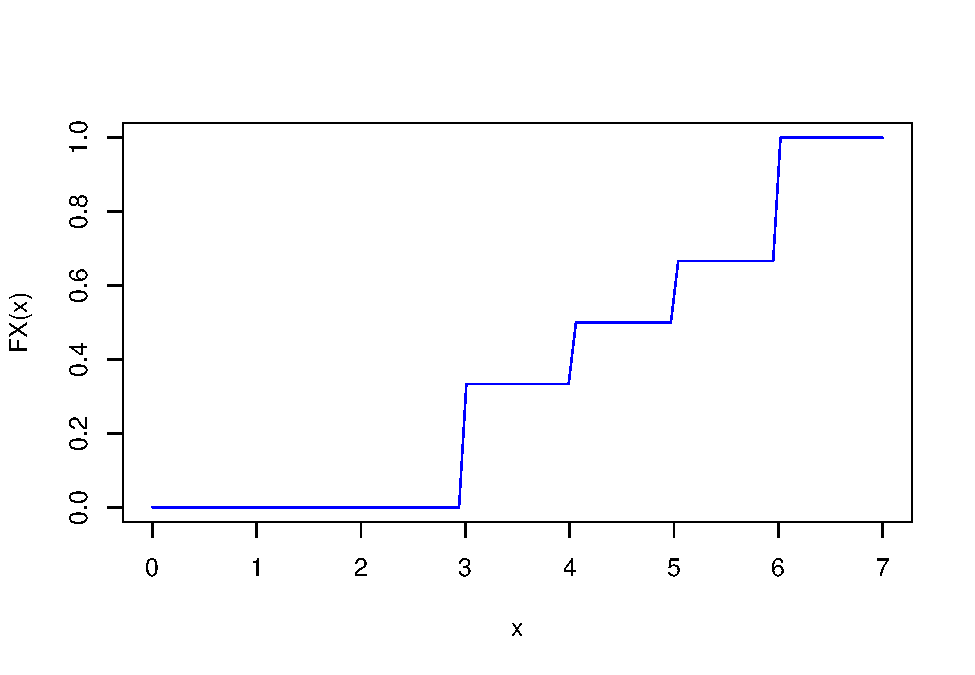
\includegraphics{Tema-2---Variables-Aleatorias_parte1_discretas_Soluciones_files/figure-latex/unnamed-chunk-2-1.pdf}

La función \(F_X\) cumple todas las propiedades de una función de
distribución discreta:

\begin{itemize}
\tightlist
\item
  \(0\leq F_X(t)\leq 1\) para todo \(t\in \mathbb{R}.\)
\item
  Es solo continua por la derecha, luego es dicreta no es continua con
  dominio \(D_X=\{3,4,5,6\}\) que son los valores dónde
  \(P(X=x)=F_X(x)-F_X(x-)\not=0\).
\item
  Tiende asintóticamente a 1 cuando \(x\to+\infty\) y a 0 cuandor
  \(x\to-\infty\).
\end{itemize}

El Dominio es \(D_X=\{3,4,5,6\}\)

\(P(X=3)=F_X(3)-F_X(3^{-})=F_X(3)-lim_{x\to 3^{-}} F_X(x)=\frac{1}{3}=\frac{1}{3}-0=\frac{1}{3}.\)

\(P(X=4)=F_X(4)-F_X(4^{-})=F_X(4)-lim_{x\to 4^{-}} F_X(x)=\frac{1}{2}-\frac{1}{3}=\frac{1}{6}.\)

\(P(X=5)=F_X(5)-F_X(5^{-})=F_X(5)-lim_{x\to 5^{-}} F_X(x)=\frac{2}{3}-\frac{1}{2}=\frac{1}{6}.\)

\(P(X=6)=F_X(6)-F_X(6^{-})=F_X(6)-lim_{x\to 5^{-}} F_X(x)=1-\frac{2}{3}=\frac{1}{3}.\)

\(P(X=x)=0\) si \(x \not\in\{3,4,5,6\}.\)

\hypertarget{problema-3.}{%
\subsection{Problema 3.}\label{problema-3.}}

La variable aleatoria \(Z\) tiene por función de probabilidad:
\[f_Z (x)=
\left\{\begin{array}{ll}
{1\over 3}, & \mbox{si $x=0,1,2$},\\ 0, & \mbox{en los otros
casos.}
\end{array}\right.
\] ¿Cuál es la función de distribución para \(Z\)?

\hypertarget{soluciuxf3n-2}{%
\subsubsection{Solución}\label{soluciuxf3n-2}}

Es discreta así que:

\[F_Z(x)=P(Z\leq x)= \sum_{z=0}^x f_Z (x)=
\left\{\begin{array}{ll}
0 & \mbox{si }  x<0 \\
{1\over 3}, & \mbox{si } 0\leq z< 1,\\ 
{2\over 3}, & \mbox{si } 1\leq z< 2,\\ 
1 & \mbox{si }  2 \leq x.
\end{array}\right.
\]

\hypertarget{problema-4.}{%
\subsection{Problema 4.}\label{problema-4.}}

Sea \(X_n\) una variable aleatoria dependiendo de un valor natural \(n\)
cuya función de probabilidad es: \[
f(x)=\begin{cases}
k\cdot i, & \mbox{si }i=1,2\ldots,n, \\
0, & \mbox{en caso contrario.}
\end{cases}
\] * Hallar el valor de \(k\) y la función de distribución de \(X\). *
Calcular la probabilidad de que \(X\) tome un valor par.

\hypertarget{soluciuxf3n-3}{%
\subsubsection{Solución}\label{soluciuxf3n-3}}

Tenemos que \(\sum_{i=1}^n k\cdot i=1\) y tenemos que determinar \(k\)
en función de \(n\), tenemos que

\[
1=\sum_{i=1}^n k\cdot i= k\cdot \sum_{i=1}^n = k\cdot \frac{n\cdot (n+1)}{2}
\]

luego

\[k= \frac{2}{n\cdot (n+1)}.\]

Nos piden \(P(X\mbox{ sea par})\) si \(n\) es par

\begin{eqnarray*}
P(X\mbox{ sea par})&=&\sum_{i=1}^{\frac{n}{2}} P(X=2\cdot i)=
\sum_{i=1}^{\frac{n}{2}}  \frac{2}{n\cdot (n+1)}\cdot 2\cdot i\\
&=& \frac{2}{n\cdot (n+1)}\cdot2 \cdot  \sum_{i=1}^{\frac{n}{2}} i=
\frac{2}{n\cdot (n+1)}\cdot2 \cdot  \frac{\frac{n}{2}\cdot (\frac{n}{2}+1)}{2}\\
&=& \frac{n\cdot (\frac{n}{2}+1)}{n\cdot(n+1)}=
\frac{\frac{n}{2}+1}{n+1}.
\end{eqnarray*}

Se deja como ejercicio el caso en el que \(n\) es impar, se tiene que
sumar

\[
P(X\mbox{ sea par})=\sum_{i=1}^{\frac{n-1}{2}} P(X=2\cdot i).
\]

\hypertarget{problema-5.}{%
\subsection{Problema 5.}\label{problema-5.}}

Un examen tipo test consta de cinco preguntas con tres posibles opciones
cada una. Un alumno contesta al azar las cinco cuestiones. Suponiendo
que cada respuesta acertada vale dos puntos, hallar la distribución de
número de puntos obtenidos por el alumno.

\hypertarget{soluciuxf3n-4}{%
\subsubsection{Solución}\label{soluciuxf3n-4}}

El dominio de la variable \(X=\) número de puntos es
\(D_X=\{0,2,4,6,8,10\}\). Calculamos primero la probabilidad de la
variables \(Y\)= número de preguntas acertadas \(D_Y=\{0,1,2,3,4,5\}\)

Prbabilidad de acertar \(n\in D_Y\) preguntas es
\(P(Y=n)={5 \choose n}\cdot \left(\frac13\right)^n\cdot \left(1-\frac13\right)^{5-n}\)

Luego

\[
P(X=x)=P\left(Y=\frac{x}{2}\right)=\begin{cases}
\left(\begin{array}{c}5\\\frac{x}{2}\end{array}\right)\cdot \left(\frac13\right)^\frac{x}{2}\cdot \left(1-\frac13\right)^{\left(5-\frac{x}{2}\right)}, & \mbox{si }x=0,2,4,6,8,10 \\
0, & \mbox{en caso contrario.}
\end{cases}
\]

\end{document}
